\begin{figure}[t]
\begin{center}
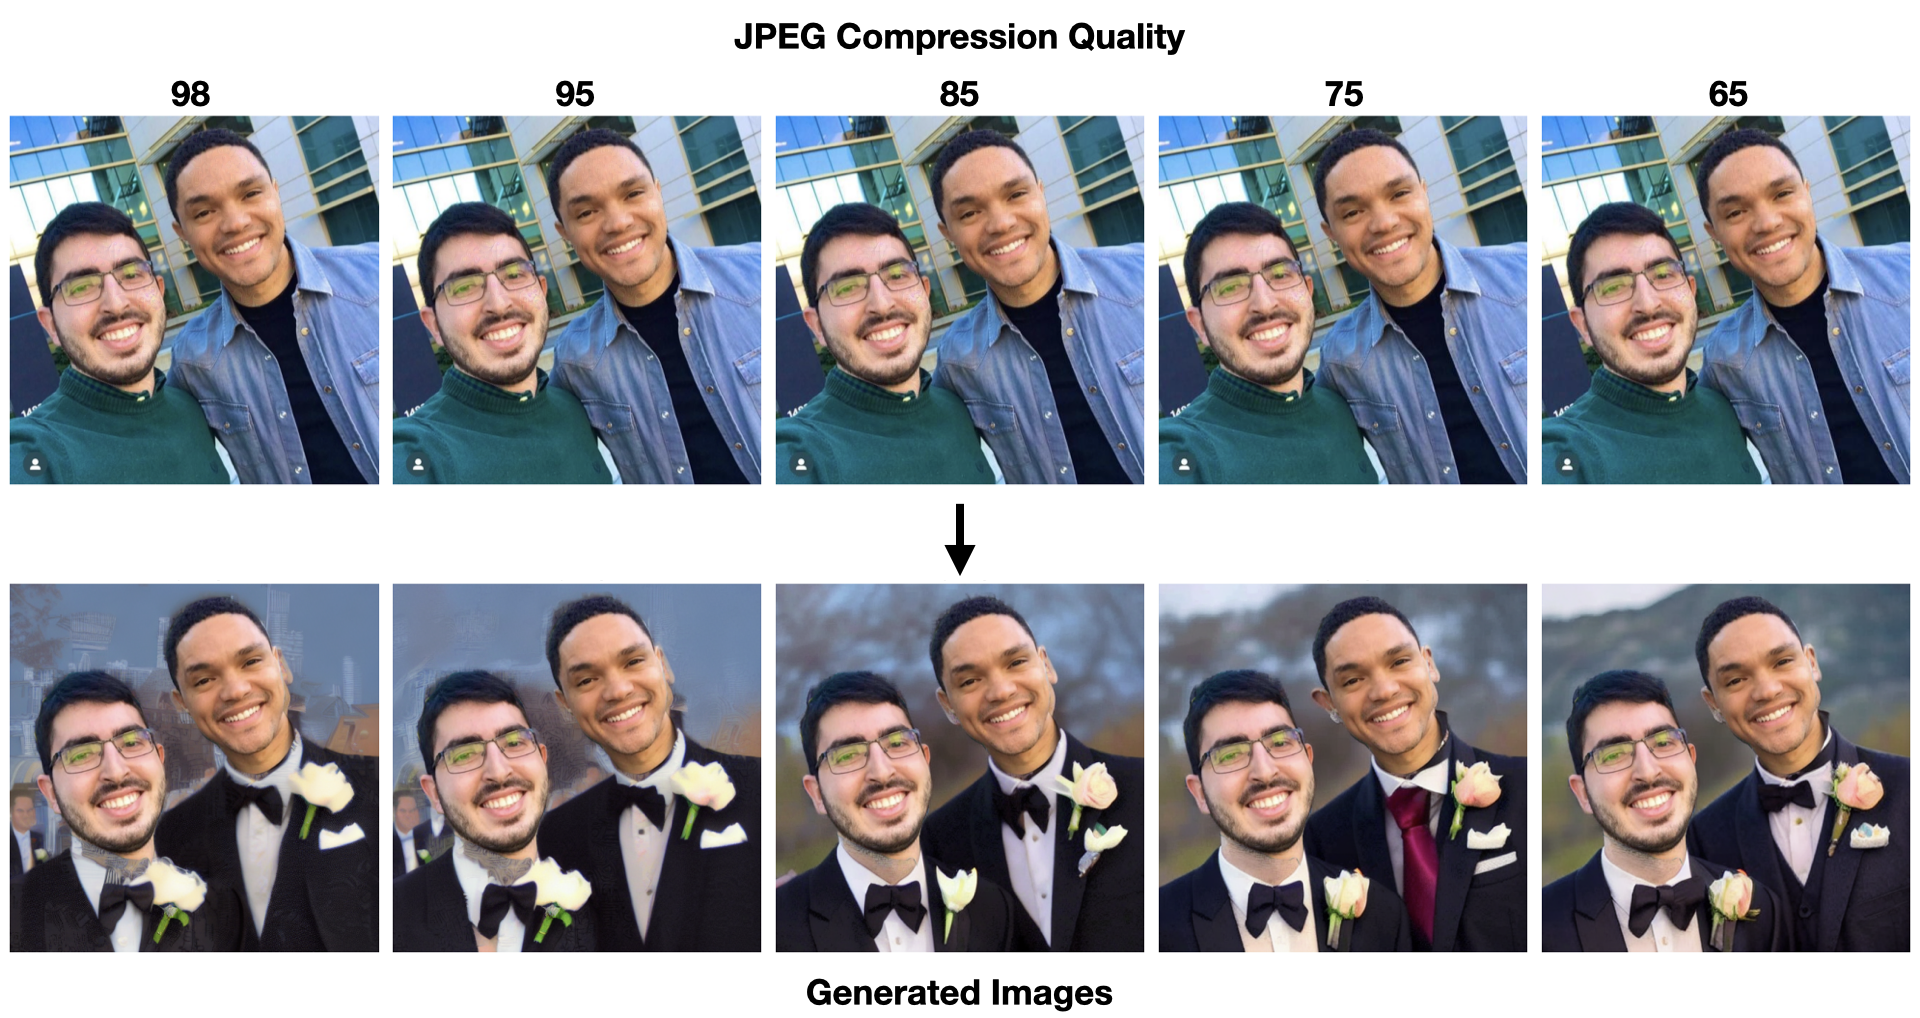
\includegraphics[width=0.75\textwidth]{images/complex-diffusion-inpaint.002.png}
\end{center}
\caption{\textbf{More JPEG compression more reliably undermines photoguard protection.} First row: We take a photoguard (Diffusion attack) image  and JPEG compress it with varying quality. Second row: Starting from the compressed image above, the adversary uses a diffusion model to make edits according to the same prompt setup as Figure~\ref{fig:inpainting-overview}. With more compression, the generated content background and clothing is more realistic. Between compression quality of 85\% and 75\%, enough of the photoguard  noise is diminished, allowing stable image edits by an adversary.}
\label{figure-jpeg-compression-inpainting}
\end{figure}